\section{Wprowadzenie}

\subsection{Istota magii}
Wiele aspektów ludzkiego życia można interpretować jako rodzaj magii. Odprawianie rytuałów, okultyzm, religię, wypowiadanie zaklęć, to można określić negatywną interpretacją magii. Bardziej pozytywnym znaczeniem magii jest określanie jej mianem emocji towarzyszącym nam w różnych sytuacjach. "Magia świąt" gdy spędzamy czas z rodziną lub gdy uczucie zakochania wpływa "magicznie"\ na nasz nastrój. Nauka nie idzie w parze z magią, mają zupełnie inne fundamenty. Podstawą nauki są badania i dowody, natomiast magia opiera się na wierze i emocjach.\par Na szczęście można połączyć naukę z magią, uzyskamy wtedy coś co nazywamy iluzją. Jest to wywołanie u widza wrażenia, iż robi się rzeczy pozornie sprzeczne z prawami fizyki poprzez zastosowanie odpowiednich trików. Każdy trik składa się z dwóch elementów. Elementu naukowego, czyli sekretu oraz elementu magicznego, czyli prezentacji.\par Sekret jest bardzo ważnym elementem triku, to on pozwala na wykonanie pozornie niemożliwej czynności. Jednakże prezentacja jest ważniejsza. To ona ukrywa nasz sekret przed publicznością, jednocześnie wprawiając ją w osłupienie.\par Prezentację można podzielić na trzy części, chociaż w znacznym stopniu się one zazębiają. Przede wszystkim iluzja ma być rozrywką, ale nie tylko dla publiczności. Magik powinien bawić się tym co robi razem z publicznością, być częścią pokazu, a nie wszystkowiedzącym guru. Kolejnym istotnym elementem prezentacji jest historyjka. Niech ma ona jakieś nawiązanie do kontekstu całej iluzji. Jeśli będzie spójna i logiczna nada większej wiarygodności całemu trikowi. Ostatnią kwestią jest umiejętność dezorientowania publiczności. Są trzy główne sposoby dezorientacji: czasowa, słowna i fizyczna. Czasowa ściśle wiąże się z historyjką. Wykorzystujemy opowiadanie, do odroczenia następnej części triku w czasie, aby publiczność zapomniała o pewnych aspektach, które się już wydarzyły. Dezoriantacja słowna polega na kłamaniu. Niekiedy wmawiamy widzowi, że zrobił coś co nie miało miejsca. Popieramy to sztucznymi rezultatami jego rzekomych działań, przez co musi nam uwierzyć. Dezorientacja fizyczna jest najprostsza z podanych. Zwracamy się do widza z prośba o wykonanie jakieś nieistotnego działania np. popukanie karty, pstryknięcie palcami. Takie czynności skupią jego uwagę, dzięki czemu sekret pozostaje bezpieczny.
\subsection{Idea triku}
Szybki postęp cywilizacyjny coraz szybciej dostarcza nam coraz lepszych urządzeń. To co kiedyś było na filmach sciencie-fiction, dzisiaj jest rzeczywistością. Ludzie nie obcujący na co dzień z takimi technologiami postrzegają je jako "magiczne pudełka", które "magicznie działają". Łatwo ich zadziwić możliwościami jakie posiada dzisiejszy smartfon. Jednakże dla osób korzystających z możliwości jakie przynoszą obecne czasy potrzeba czegoś więcej. Można skorzystać z technologii, której możliwości nie znają. Wpadliśmy na pomysł wykorzystania jednej z dostępnych funkcji systemu operacyjnego Android, NFC. Do triku należy przygotować:
\begin{itemize}
    \item Pytajnik - kastomowa karta ze wzorem białego znaku zapytania na czerwonym tle

\includegraphics[scale=0.04]{imgs/pytajnik.PNG}. Wzór pytajnika może zostać nadrukowany na dowolnym materiale. Nam zależało na długiej żywotności, więc zleciliśmy nadrukowanie wzoru na plastikowej karcie.
    \item Talię - talia kart z wklejonymi naklejkami NFC. Talię można zlecić do wykonania drukarni lub wykonać własnoręcznie naklejając tagi na rewers kart. Nam udało się osiągnąć bardzo dobry efekt, ze względu na dopasowanie fragmentu rewersu do kształtu znacznika.
    \item Aplikację - poprawnie skonfigurowana aplikacja Technologic na smartfonie z Androidem w wersji conajmniej Lollipop. Wartości zapisane do tagów na konkretnych kartach muszą się zgadzać z tymi w aplikacji. Ponadto należy wybrać, który wariant triku wybieramy (Fotografia/Wibracje).
    \item Woreczek - ciemny, nieprzeźroczysty woreczek wielkości karty do gry.
    \item (opcjonalnie) Pokrowiec - pokrowiec na telefon, który nie przekazuje gestów z zewnątrz.
    \item (opcjonalnie) Schemat wibracji - dla każdej karty ustalić sześciobitowy ciąg. Zaleca się, aby pierwsze dwa bity określały kolor, a pozostałe cztery wartość, jednakże nie jest to obowiązkowe. Jedynka jest sygnalizowana jedną krótką wibracją, natomiast zero dwoma krótkimi wibracjami.
\end{itemize}

\paragraph{Konfiguracja}\mbox{}\\
\begin{figure}[H]
\centering
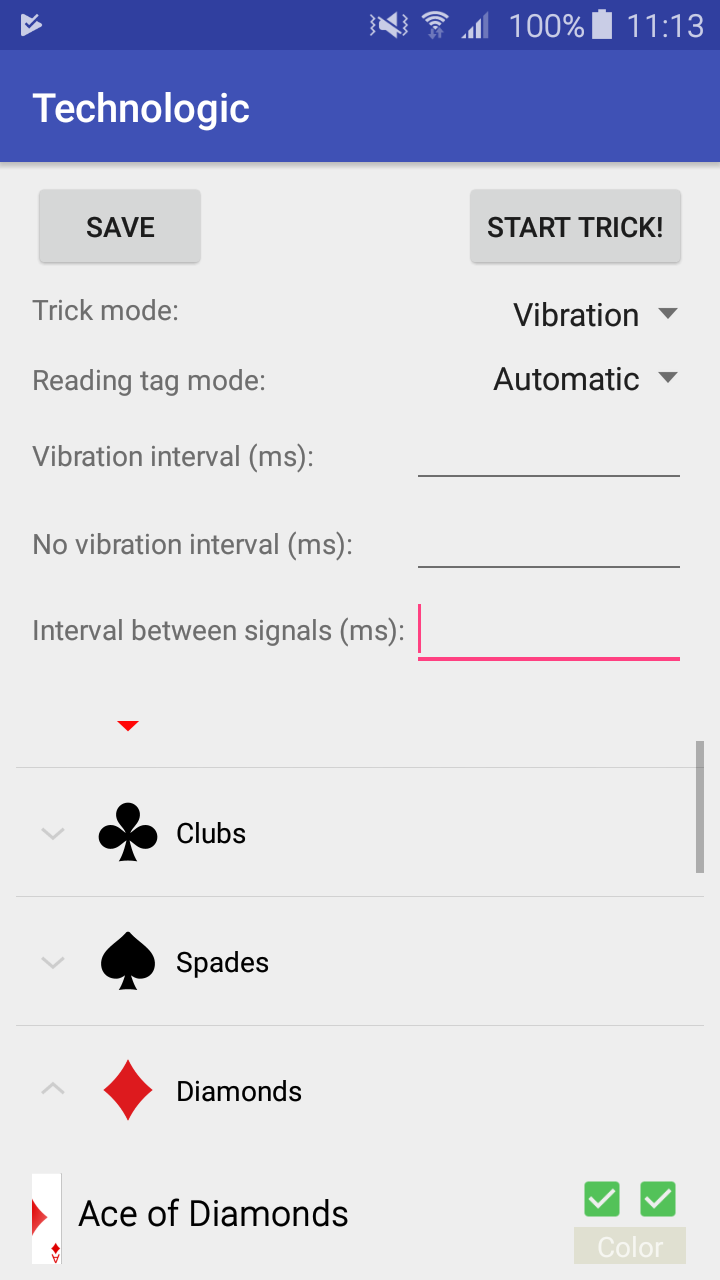
\includegraphics[scale=0.22]{imgs/mainActivity.png}
\caption{Panel konfiguracyjny aplikacji}
\end{figure}
Przycisk \textit{START TRICK!} uruchamia Aktywność określoną w opcji \textit{Trick mode}. Dostepne są trzy możliwości: tryb zapisywania wartości do znaczników oraz dwa rodzaje odczytywania (Fotografia lub Wibracje). Opcja \textit{Reading tag mode} ma dwie możliwości do wyboru, automatyczny lub manualny. Odpowiada to za operacje związane z NFC, mogą się one wykonywać automatycznie po wykryciu tagu lub na żądanie poprzez wciśnięcie przycisku. \textit{Vibration interval} odpowiada za długość (w milisekundach) trwania pojedynczej wibracji. \textit{No vibration interval} to długość (w milisekundach) odstępu między dwoma wibracjami, gdy sygnalizujemy wartość 0. \textit{Interval between signals} to długość (w milisekundach) trwania przerwy między sygnalizowanymi bitami. Każda z grup koloru kart ma elementy, które zawierają informacje na temat nazwy oraz schematu wibracji kolejnych kart. Nazwę karty podajemy w polu tekstowym znajdującym się po prawej stronie od ikony reprezentującą tę kartę, natomiast schemat wibracji ustalamy za pomocą pól wyboru. Dla ułatwienia mają one podpis, które z nich odpowiadają za kolor, a które za wartość karty. Przycisk \textit{SAVE} służy do zapisania ustawień do pliku, dzięki czemu będą one się automatycznie ładować przy starcie aplikacji. 
\par
Po przygotowaniu wszelkich niezbędnych elementów, możemy przystąpić do wykonywania triku. Smartfona z aplikacją chowamy do kieszeni. Aplikacja musi być na pierwszym planie i urządzenie nie może być zablokowane. Zaleca się skorzystanie z pokrowca, aby aplikacja przez przypadek nie przeniosła się na inny plan. Wybieramy widza z publiczności, podajemu mu talię i prosimy go o przetasowanie kart. Następnie prosimy go o wybranie dowolonej karty z talii, zapamiętaniu jej i umieszczeniu w woreczku. Odbieramy od niego resztę talii, a woreczek wkładamy dyskretnie do kieszeni (w tym momencie aplikacja odczytuje zawartość ze znacznika). Dalszy przebieg występu zależy od wybranego wcześniej wariantu. Kluczowym działaniem dla obu wariantów jest dezorientacja czasowa w postaci historyjki.
\paragraph{Fotografia}\mbox{}\\


% \noindent\textbf{\large{Fotografia}}\par
Możemy odłożyć karty, nie będą potrzebne. Ten wariant można zakończyć na dwa sposoby. W zależności od wybranego zakończenia będzie zastosowana inna historyjka. \par 
Pierwszą opcją jest zrobienie zdjęcia portretowego widzowi za pomocą aplikacji. Na fotografii zostanie umieszczony obrazek ze wzorem karty widza na wysokości jego czoła. Historyjką dla tego zakończenia mogłoby być: "W dzisiejszych czasach technologia coraz bardziej ingeruje w ludzki umysł. Nie orientujemy się kiedy urzędzenia czytają nam w myślach upraszczając nam codzienne życie. O ilu rzeczach nie musimy pamiętać, ponieważ coś robi to za nas. Mój smartfon również posiada taką możliwość. On umie czytać w myślach! Nie wierzycie? Pozwólcie, że zaprezentuję (...)"\par
Drugą opcją jest podanie widzowi pytajnika. Następnie robimy dowolne zdjęcie widzowi, w taki sposób, aby pytajnik był widoczny. Na fotografii, obraz pytajnika zostanie zastąpiony obrazem ze wzorem karty widza. W tym przypadku historyjką mogłoby być: "Teraz drodzy Państwo chciałbym Wam przedstawić magiczną kartę. Jest bardzo skryta, a swoją wartość trzyma wewnątrz siebie i nieczęsto ukazuje ją światu. Jednakże jest bardzo podatna na sławę, wtedy ujawnia swoją tajemnicę. Spróbujmy nagrodzić ją brawami, a Pan/Pani niech jej powie, że jest jej największym fanem i zapozuje z nią do zdjęcia. Będę paparazzi! (...)"\par
W obu sytacjach efektem triku jest fotografia, na której widnieje karta widza. Można ją wysłać widzowi na pamiątkę, gdyż znajduje się ona w pamięci smartfonu w folderze Technologic.
\paragraph{Wibracje}\mbox{}\\
Ten wariant jest trudniejszy i wymaga pewnych umiejętności od magika. Talię można zostawić przy sobie, gdyż może się przydać do odgadywania karty. Po umieszczeniu woreczka z kartą w kieszeni, smartfon zacznie wibrować przekazując konkretny schemat wibracji ustalony wcześniej w aplikacji. Dzięki znajomości schematu, jesteśmy w stanie wywnioskować jaką kartę wybrał widz. Historyjką do tego zakończenia mogłoby być: "Wielu magików odnajduje wybrane karty w różnych miejscach, które wydają się niemożliwe. Ja natomiast odnajdę kartę w miejscu gdzie jej nie ma! Będę wykładać odkryte karty na stół i na ich podstawię powiem jakiej karty brakuje w talii!". Podczas wykładania kart, nie należy grupować kart w jeden stosik. Niech z kart ułoży się wzór  odpowiadający wartości karty znajdującej się w kieszeni. To sprawi wrażenie, że od momentu wykładania kart na stół wiedziałeś jakiej karty brakuje.\par
Po zakończeniu triku w pierwszym wariancie nie należy chować telefonu do kieszeni z woreczkiem. Najlepiej odłożyć go gdzieś lub ewentualnie schować do innej kieszeni. W drugim wariancie natomiast nie należy wyciągać telefonu z kieszeni, aby uniknąć podejrzeń.
